\chapter{Graph Laplacian Embedding}


\subsection{Manifolds}
\label{sec:manifolds}

\textbf{TODO:
it maps Rd to RD, if d<D. 
In our case, it map an angle in S1 (subset of R) to something in RM. The circle S1, is 1 dimensional, 
it depends only on 1 parameter, and can be represented in R2 like you did. 
I thinks (not 100 of sure of that right now) that the  rotation group is a manifold, 
it maps 1d parameter (rotation angle) to some rotation operator (which is high dimensional)
we don't calculate manifold. 
Diffusion maps (or graph Laplacian embedding) are a way to map high dimensional dataset to low dimensional one. 
When the data points are sampled from a manifold, the GL embedding is closely related to the manifold itself.
We can expect the GL embedding to share property of the original manifold, such as preservation of distances between points}


In high-dimensional data Euclidean distances are not meaningful
in the sense that they will not capture similar data points well. 
Graph Laplacian can be used to compute a \textit{Manifold}, which can help in such scenarios. 
In manifold space, Euclidean distances make sense again. 
Let manifold $M$ be defined as $\mathcal{M} = \{ f(x), f \in C^K, f: \mathbb{R}^D \to \mathbb{R}^d \}$.
Manifolds are a well established mathematical concept. In the Master's Thesis, only 
$C^k$ differentiable d-dimensional manifolds defined by $\mathcal{M}$ are considered. 
When $d \ll D$, manifolds define a \textit{low-dimensional embedding}, which maps from high-dimensional space 
$\mathbb{R}^D$ to low-dimensional space $\mathbb{R}^d$.

Let's give two popular examples of manifolds, namely the \textit{circle} and the \textit{sphere}.
The circle is a 1D manifold, where $d=1$ and $D=2$. A sphere is a 2D manifold with $d=2$ and $D=3$.
In Figure~\ref{fig:circle_sampling}, 200 samples are drawn from a uniform distribution of the unit-circle manifold
and in Figure~\ref{fig:sphere_sampling}, 800 samples are drawn from a uniform distribution of the unit-sphere manifold,
as well as the sphere itself.

\begin{figure}[H]
    \hfill
    \subbottom[
        \label{fig:circle_sampling}]
        {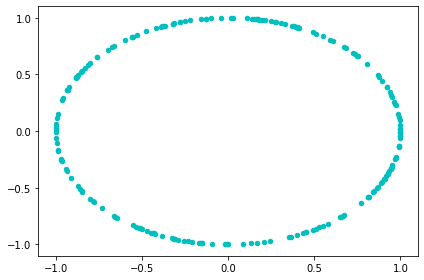
\includegraphics[width=0.4\textwidth]{circle_sampling.png}}
    \hfill
        \subbottom[      
    \label{fig:sphere_sampling}]
        {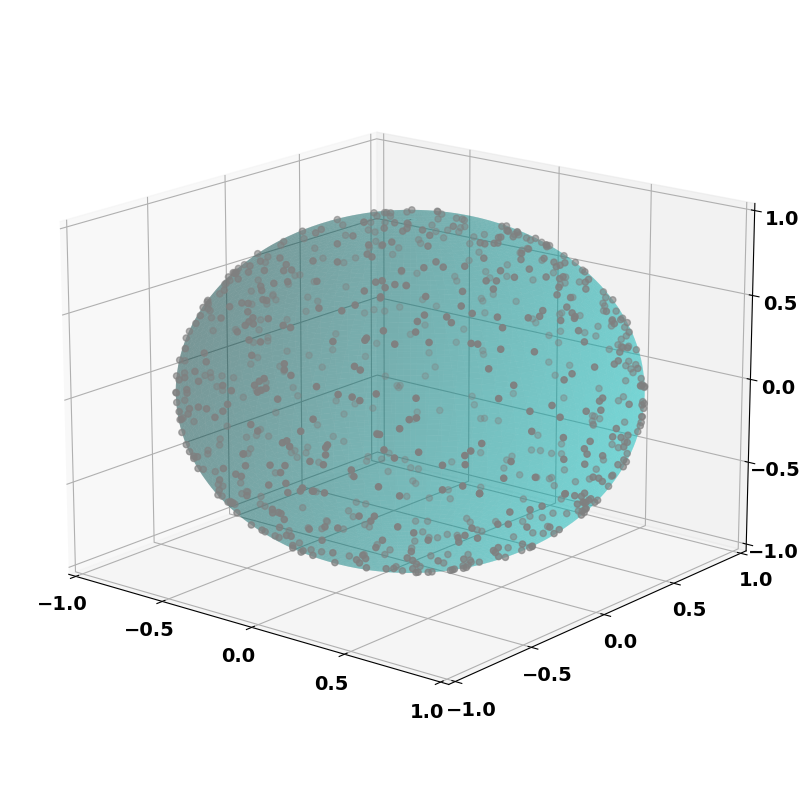
\includegraphics[width=0.42\textwidth]{sphere_sampling.png}}
    \hfill
        \caption{Samples drawn from 1D and 2D manifold: 
    \ref{fig:circle_sampling} circle samples,
    \ref{fig:sphere_sampling} sphere samples}
\end{figure}

One popular algorithm for calculating manifolds is diffusion maps~\cite{diffusionMaps}, 
which is a non-linear approach for calculating low-dimensional manifolds
for (high-dimensional) datasets, using Graph Laplacian.
Vector diffusion maps~\cite{vectorDiffusionMaps} generalize the concept of diffusion maps for vector fields.
Multi-frequency vector diffusion maps~\cite{multiDiffusionMaps} 
can be seen as an extension to vector diffusion maps, which works well even on highly noisy environments.
\citet{cryoEmMutliDM} successfully applied multi-frequency vector diffusion Maps in cryo-EM setting,
 where it was used for denoising observations.

\subsection{Manifold assumption}
\label{sec:manifoldAssumption}
Manifold assumption is a popular assumption for high-dimensional datasets.
For a given dataset in high-dimension, one can assume that data points are samples drawn from a low-dimensional manifold,
that embeds the high-dimensional space. 
Therefore, if underlying manifold can be approximated, a dimensionality reduction
is established as one can embed data points in the low-dimensional manifold space.
There is a complete area of research devoted to this manifold assumption called Manifold Learning\cite{ManifoldLearning}.

\subsection{GL-manifold calculation}
\label{sec:manifold_calculation}
A simple low-dimensional embedding (manifold) of a dataset can be calculated with Graph-Laplacian 
by the following:

\begin{enumerate}
    \item Construct k-NN graph from observations (see Section~\ref{sec:graphConstruction} \textit{\nameref{sec:graphConstruction}}).
    \item Calculate the (normalized) Graph Laplacian (see Equation~\ref{eq:gl}).
    \item Extract the second, third (and fourth) the smallest eigenvectors.
\end{enumerate}